The slow extraction of the beam is controlled via the RF-Knock out (RFKO) technique. This allows a precise and reproducible intensity control spill by spill.

An RFKO extraction process involves using a transverse beam disturbance with a noise signal whose frequency changes over time (frequency modulation (FM)). This change in frequency is necessary to affect all particles. We do a sweep - or chirp - in frequency. 

With the noise from the chirp, the particles are diffused from the beam core to the stable triangle.

\begin{figure}[h]
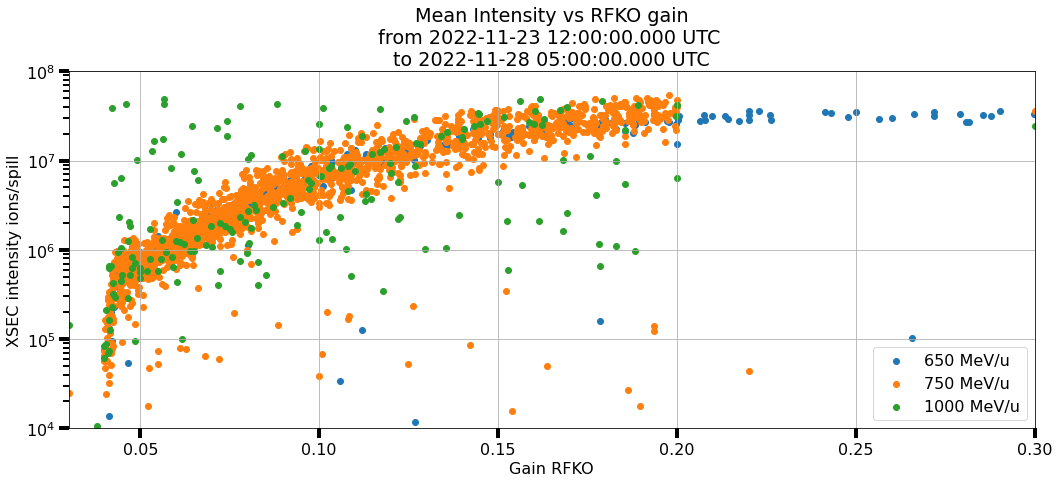
\includegraphics[width=0.9\textwidth]{images/xsec70_intensity_vs_gain.png}
\end{figure}

The RFKO has different parameters to control the extraction:
- Chirp gain: the voltage applied to the RFKO plates.
- Chirp frequency range
- Accuracy (number of turns in the PS)
- Bounds: Start and stop of the chirping

Lowest chirps is 512 turns
Time it takes for one turn in the PS = **2.1 $\mu s$**
* $t = \frac{circumference}{c} = \frac{628}{3e8} = 2.1e-6 [s]$

5.12e2 * 2.1e-6 = 1.752e-3 s = 1.8 ms

\begin{figure}[h]
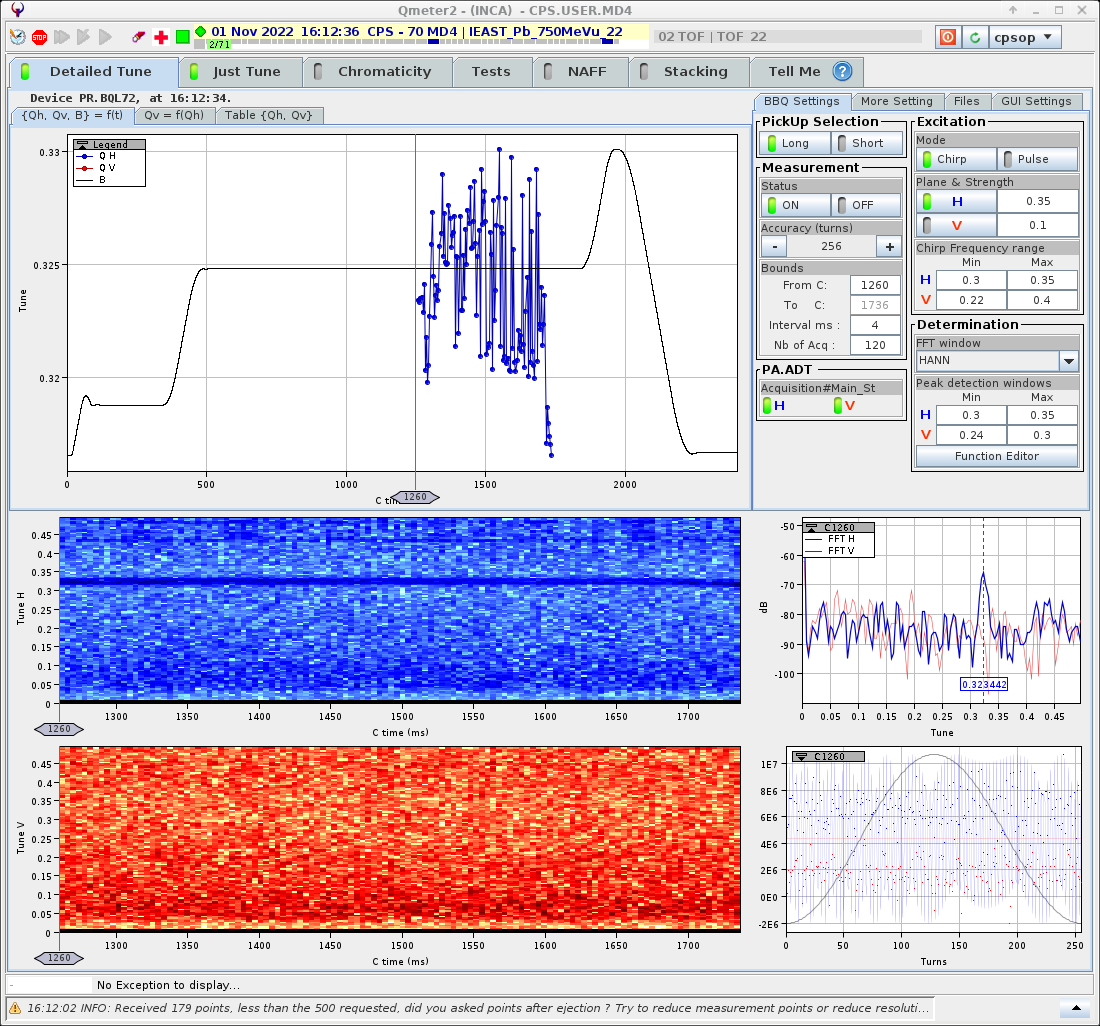
\includegraphics[width=0.4\textwidth]{images/qmeter.png}
\end{figure}

\begin{figure}[h]
\centering
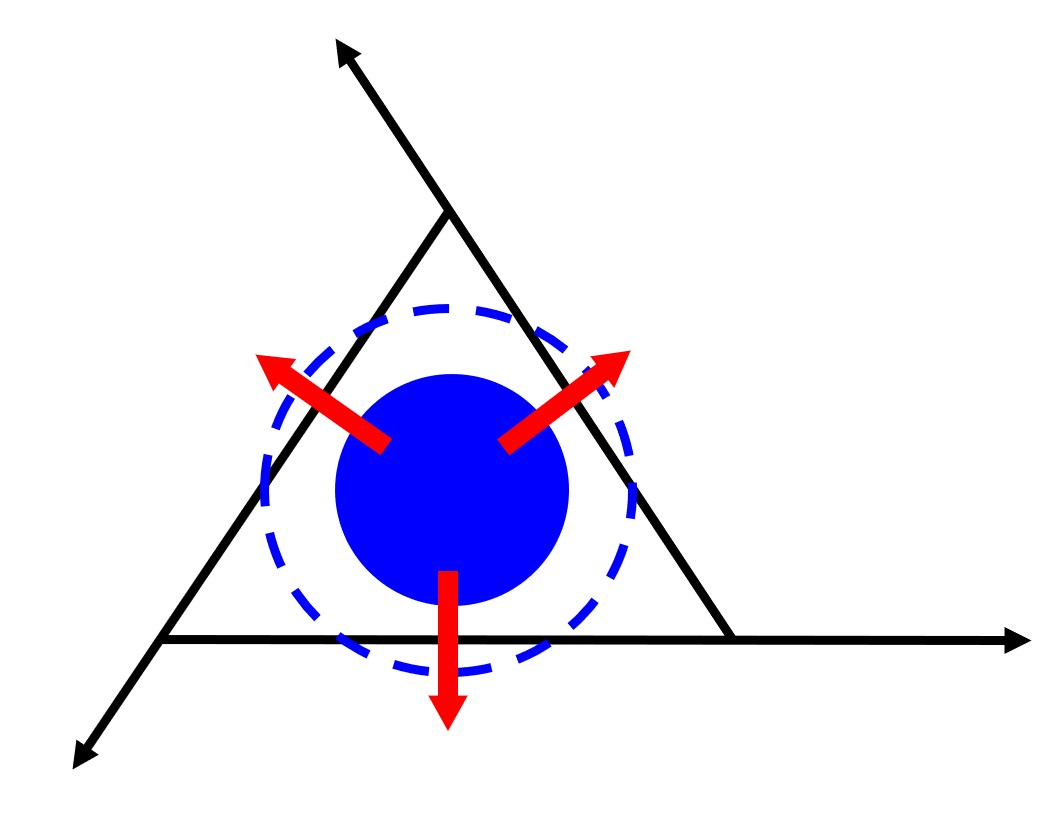
\includegraphics[width=0.4\textwidth]{images/RFKO.jpg}
\end{figure}